\documentclass{amsart} 
\usepackage{graphicx}
\graphicspath{{./}}
\usepackage[fontsize=14pt]{scrextend}
\usepackage{hyperref}
\title{Truths about Human Race versus Far Right Racist Myths}
\author{Zulfikar Moinuddin Ahmed}
\date{\today}

\begin{document}
\maketitle

\section{Far Right are Lower IQ than Mainstream}

I am not white, so I can't tolerate denigrating comments from idiots about racial supremacy theories, especially given that my IQ is 135-140 (SAT was 1450 and I graduated valedictorian of John Adams High School in New York 1991) and I have to hear about white superiority from these idiots when white IQ is $N(100,15)$ and I am in the 99.6th percentile of this distribution.  A published study \cite{HB} from 2012 showed correlation between low IQ and racist views.

S. Kanazawa did a study estimating IQ from adolescents and political positions in young adulthood and found 11.6 difference in IQ between very conservatives and very liberal people.  

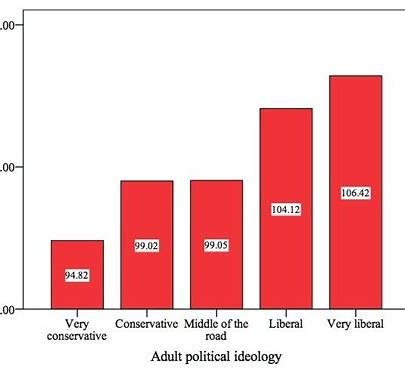
\includegraphics[scale=0.8]{kanazawa.jpeg}

\section{Truth about Human Race}

Sewall Wright already had enormous amount of experimental data to refute the theory of multiple biological races in humans.  His index of fixity measured $F_{ST} < 0.15$ across continental groups; this has been refined to $F_{ST} < 0.12$ in a 2012 study.  Around 75,000 years ago all non-African humans originate from a meta population in East Africa.  Therefore the Human Race is a single race with an estimate of how long ago we were part of the same tribe.  

Given this truth, the inability for some in the far right to accept other people and consider themselves a higher race and so on is a function of low intelligence.  To be blunt, it is the lack of education and ignorance in current scientific literature that allows far right racists to hold on to various racist prejudices.  This is something that is not spoken about clearly in our American public sphere.  I am not so charitable at 48 towards variable viewpoints on issues where science has been quite thorough and clear.  Then it's no longer a matter of political preference any more but a matter of public education and a public safety hazard.  This is not a joke.  I have been physically assaulted by white racists in America multiple times.  People who propagate this rubbish ought to be taken to jail.

\section{Classical Liberalism does not allow Falsehoods in Freedom of Speech}

Classical Liberal philosophy which underlies all politics in America does provide protections for individual liberty and freedom of speech.  At the same time, the philosophy also respects Truth as an ideal.  

Let me give an artificial scenario to illustrate my point.  Suppose you go to the grocery store and pick \$2 milk and \$3 bread and the machine adds it up and charges you \$2,000.  Then you complain to the store-owner and he does not budge and claims that the machine used Freedom of Speech where $2 + 2 = 2000$.  This is disallowed by Classical Liberalism.  

This argument then applies to multiple race theories.  Since science has established without much doubt that the truth is that there is a single human race and separate biological races are fiction, those who propagate racial supremacy theories ought to be found in violation of Truth and be held accountable despite their Freedom of Speech.  Freedom of Speech is not meant for blatant falsehoods.

\section{Classical meaning of superiority}

Classically 'superiority' has never been about race in high culture.  Primarily it has been about superiority in moral Character and Conscience.  I recently had great conflict with a wealthy white man in industry who holds the view that 'whites are superior' and when presented with the fairly clear records of on average from 1985-2019 around 2600 white people arrested for murder charges, fairly blatant failure of moral virtues, which would lead to the elementary inference that these particular white people are morally {\em inferior} to all non-whites who are not murderers, his reaction was to dismiss FBI measurement of the data professionally collected as "PR".  

Let me repeat this clearly, when we compare groups of people, one group all white and another group all non-white, and use moral Character as the ordering, Reason demands that we find all the non-white non-murderers superior to all the white murderers.  This is an elementary exercise that is not done enough when people are pretending to be charitable towards non-whites in public with the hidden belief that this is just a 'politically correct' facade to hold egalitarian views in public.  In fact, white murderers are inferior to non-murderers both white and non-white.  There is no political correctness involved here.  And in America roughly 2600 murders a year are committed by white murderers.  In 2018 there were 3,011 murders committed by white people \cite{FBI18}; and 3177 murders were committed by black people.  And non-white murderers are inferior to both white and non-white murderers.  

People who are murderers and rapists are morally inferior to those who are not murderers and rapists; plenty of these are non-white but a significant percentage are in fact white.  This significant fraction of morally inferior whites seem to disappear from the conversation when the topic appears in public sphere.

This elementary point has a natural elementary reasonable position, that we do not have prejudice against people and their moral character based on white or non-white.  That is the rational position, not the {\em politically correct position}.


\begin{thebibliography}{CCC}
\bibitem{HB}{Hodson, G. and Busseri, M.A. (2012). Bright minds and dark attitudes: Lower cognitive ability predicts greater prejudice through right-wing ideology and low intergroup contact. Psychological Science, 23, 187--195}
\bibitem{K10}{S. Kanazawa, Why Liberals and Atheists are More Intelligent, Social Psychology Quarterly, 2010  73 (1) 33--57.}
\bibitem{FBI18}{\url{https://ucr.fbi.gov/crime-in-the-u.s/2018/crime-in-the-u.s.-2018/tables/expanded-homicide-data-table-6.xls}}
\end{thebibliography}
\end{document}